% Intended LaTeX compiler: pdflatex
\documentclass[10pt,a4paper,UTF8]{article}
\usepackage{zclorg}
\usepackage{tikztheorem}
\author{zcl.space}
\date{}
\title{Limits}
\hypersetup{
 pdfauthor={zcl.space},
 pdftitle={Limits},
 pdfkeywords={PMA},
 pdfsubject={},
 pdfcreator={Emacs 25.0.50.1 (Org mode 9.1.2)},
 pdflang={English}}
\begin{document}

\maketitle
\tableofcontents
\titlepic{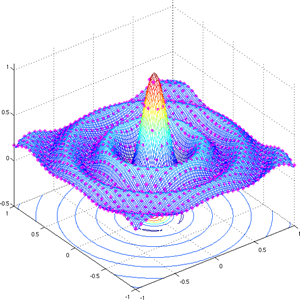
\includegraphics[scale=0.25]{../../img/sinc.PNG}}
The intuitive idea of the notation
$$
   \lim_{p\to p_0}F(p) = L
$$
is that \(F(p)\) is very close to \(L\) when \(p\) is very close to \(p_0\).
Some authors write \(F(p)\to L\) as \(p\to p_0\);  others write
\(F(p)\approx L\) when \(p\approx p_0\). In this chapter we give a more precise definition.
The following lingo is helpful.

 A set \(U\) is called a \textbf{neighborhood} of the point \(p\) if \(U\) contains some
open ball \(B(p,\delta)\) centered at \(p\).
A \textbf{punctured neighborhood} of \(p\) is
a set of form \(U\setminus\{p\}\) where \(U\) is a neighborhood of \(p\).

A point \(p\) is a \textbf{accumulation point} of a set \(S\)  iff every punctured neighborhood of  \(p\) contains a point of \(S\).
The following equivalent definition appears in some books.

\begin{tikztheorem}
A point \(p\) is an accumulation point of the set \(S\) if and only if every neighborhood
of \(p\) contains infinitely many points of \(S\).
\end{tikztheorem}

\begin{proof}
 ''If'' is easy: an infinite set is nonempty and at most one of the points
in an infinite set is \(p\). For ''only if'' assume
\(p\) is an accumulation point of the set \(S\) and choose a neighborhood \(U\) of \(p\).
By definition there is a point \(p_0\in U\cap S\setminus\{p\}\). Let \(\delta_0=|p-p_0|\).
For \(n>0\)
define \(\delta_n>0\) and \(p_n\in S\) inductively  by \(\delta_n=\min(|p_n-p|,1/n)\) and
\(p_{n+1}\in B(p,\delta_n)\cap S\).
The map \(n\mapsto p_n\) is injective as \(|p_n-p|<|p_m-p|\) for \(n>m\).
Choose \(\delta>0\) so that \(B(p,\delta)\subset U\) (by the definition of neighborhood).
Then \(\delta_n<\delta\) for \(1/n<\delta\) so \(p_n\in B(p,\delta)\cap S\subseteq U\cap S\).
Hence \(U\) contains the infinite set  \(\{p_n:n>1/\delta\}\).
\end{proof}

Let \(p_0\) be a accumulation point of a set \(S\) and \(F\) be a function defined on
\(S\) (but possibly not at \(p_0\)). The notation
\begin{equation*}
\label{eq:1}
   \lim_{p\to p_0}F(p) = L
\end{equation*}


means that
for every  neighborhood \(V\) of \(L\) of there is a punctured neighborhood \(U\setminus\{p\}\) of \(L\)
such that \(f(S\cap U\setminus\{p\})\subset V\).
When \(p_0\in S\) and \(p_0\) is a accumulation point of \(S\) we have that
a function \(f\) defined on \(S\) is continuous at \(p_0\)
if and only if
$$
\lim_{p\to p_0}f(p) =f(p_0)
$$
(and the function is  trivially continuous at a point \(p_0\in S\) which
is not an accumulation point of \(S\)).
However, the limit notation is usually used in situations where
(\(p_0\) is a accumulation point of \(S\) but) \(p_0\notin S\).
For example,
the \jdef{derivative} of a real valued function \(f:I\to\mathbb{R}\)
defined on an open interval \(I\subseteq\mathbb{R}\) is defined by
$$
f'(x_0):=\lim_{x\to x_0}\frac{f(x)-f(x_0)}{x-x_0}.
$$
The ratio in the limit is undefined when \(x=x_0\)
but is defined  for nearby values of \(x\).


For a real valued function \(f\) defined on a subset of \(\mathbb{R}\)
we can extend the definition of the notation
\(\lim_{x\to a}F(x)=L\) to include the cases where \(a=\pm\infty\)
and/or \(L=\pm\infty\) as follows.  Let

\[\hat{\mathbb{R}}:=\{-\infty\}\cup{\mathbb{R}}\cup\{\infty\}\]

consist of the set of real numbers together with two additional
points which we think of as located at infinity. The set \(\hat{\mathbb{R}}\)
is sometimes called the set of \textbf{extended real numbers}.
Extend the usual order relation on \(\mathbb{R}\) to \(\hat{\mathbb{R}}\) in the obvious way.
For \(a\in\hat{\mathbb{R}}\), a set \(U\subseteq\hat{\mathbb{R}}\) is called
\textbf{neighborhood} of  \(a\) iff

\begin{enumerate}
\item either \(a\in\mathbb{R}\) and \(U\) contains an open interval \((a-\delta,a+\delta)\) for some \(\delta  >  0\),
\item or else \(a=\infty\) and \(U\) contains an interval \((M,\infty]\) for some \(M > 0\),
\item or else \(a=-\infty\) and \(U\) contains an interval \([-\infty,-M)\) for some \(M > 0\).
\end{enumerate}


Because \(B(a,\delta)=(a-\delta,a+\delta)\) this definition agrees
with the definition  of \textbf{limit} for \(a\in\mathbb{R}\).
A point \(a\in\hat{\mathbb{R}}\) is called a \textbf{accumulation point} of a subset \(S\subseteq\mathbb{R}\)
iff every punctured neighborhood of \(a\) intersects \(S\).
If \(f:S\to\mathbb{R}\) and \(a\) is a accumulation point of \(S\), then the notation
$$
     \lim_{x\to a} F(x)=L
$$
means that for every neighborhood \(V\) of \(L\) there is a punctured neighborhood
\(U\) of \(a\) such that \(f(U\cap S)\subseteq V\).


Unraveling the above definitions we see that for \(a,L\in\mathbb{R}\)  we have that
\(\lim_{x\to a} F(x)=L\) iff \(\forall \epsilon > 0\,\exists \delta > 0\) such that \(\forall x\in S\)
we have that \(0 < |x-a| < \delta\implies |F(x)-L| < \epsilon\). Also \(\lim_{x\to\infty} F(x)=L\) iff \(\forall \epsilon > 0\,\exists M > 0\) such that \(\forall x\in S\) . we have that  \(M < x\implies |F(x)-L| < \epsilon\)
with similar definitions for the other cases where \(a,L\in\{\pm\infty\}\).

The various definitions given in \textbf{limit} and \textbf{extended\_reals} are easier
to understand because the lingo makes them look the same and because there aren't so
many symbols. This is why the terminology was invented.
\end{document}
